\chapter{Asking Billionaires How They Got Rich! (New York)}

This School of Hard Knocks interview, curated here by LazyingArt LLC, is not a lecture in the classroom sense, but it does have a mathematical spine. The host keeps asking the same small set of questions, and the answers repeatedly collapse into quantities, thresholds, time horizons, and update rules: annual sales, years in business, starting capital, leverage through rent, bank returns, long-horizon compounding, and the control problem of delegation. The safest way to write the chapter is therefore to follow the lecture's own order. We begin with a teaser of scale, reset the frame on Billionaires Row, move through construction, shoes, real estate, and trading, and only then draw out the shared logic.

\section{Cold Open and Billionaires Row}

The lecture opens by spending consequences before causes. We are shown, in compressed form, a billionaire shoe founder, a trader who says Amazon was his cash cow, and several large money numbers before the host formally explains the setting. The numerical preview is already enough to tell us what sort of chapter this will be:
\begin{align}
R_{\text{SM}} &\approx \$2.5\,\text{billion/year},\\
Y_{\text{operator}} &\approx \$12\text{--}15\,\text{million/year}.
\end{align}
At this point these are not yet arguments. They are endpoints.

Only after the teaser does the host reset the frame: we are on Billionaires Row, on the richest street in New York, and the project is to walk the street and recover blueprints rather than merely admire outcomes. That reset matters. It converts spectacle into experiment. We are not just being told that wealth exists; we are being promised that repeated street encounters will uncover what sorts of mechanisms wealthy operators actually trust.

\section{Construction, Inspection, and the Negative Art of Selling}

The first fully developed interview is with a construction mogul. The early part of the exchange establishes scale. He says he has never been broke, has owned a company for decades, builds towers from Philadelphia to Miami, and gives both a personal and a business-side annual figure:
\begin{align}
t_{\text{construction}} &= 35\,\text{years},\\
Y_{\text{construction,personal}} &\approx \$30\,\text{million},\\
R_{\text{construction,max}} &\approx \$200\text{--}500\,\text{million/year}.
\end{align}
The last line has to be kept rough. The transcript moves from ``several hundred'' to probing around \(\$200\) million and \(\$500\) million, and the final answer is only ``in that area.''

What matters next is not the size but the control doctrine. Asked for the best financial advice he ever received, he says: stay involved. The host immediately poses the obvious objection. Does that not trap us in the business rather than above it? The speaker's answer is sharper than the slogan. Delegation is not the problem. Uninspected delegation is the problem. In his own phrasing, people respect what we inspect.

We may compress that rule into a simple implication:
\begin{equation}
\text{delegation} + \text{inspection} \Rightarrow \text{maintained control}.
\end{equation}
That formula is not a literal theorem from the interview, but it captures the mechanism. The company may be distributed, but the operator must still sample reality often enough that subordinates know standards are live.

The lecture then shifts from operating control to diversification. The same speaker lists several business lines,
\begin{equation}
\mathcal{B}_{\text{mogul}}=
\{\text{real estate},\ \text{manufacturing},\ \text{construction}\},
\end{equation}
and explicitly rejects the common startup slogan that one must focus on only one thing forever. This is not presented as a universal law; it is a speaker's style of wealth-building, and the chapter should keep it in that speaker-attributed register.

The final move in the interview is the most conceptually interesting one. Asked about sales, he first says he knows how to close a deal, then immediately refines the statement: the real secret is knowing what deal not to do, and even whom not to talk to. That is a different picture of selling. We are not merely pushing toward yes; we are pruning away bad counterparties and bad situations.

A concise formal summary is
\begin{equation}
\text{bad deal avoidance} + \text{counterparty filtering} \Rightarrow \text{sales edge},
\end{equation}
with its darker counterpart
\begin{equation}
\text{greed} + \text{desperation} \Rightarrow \text{wrong deal entry}.
\end{equation}
The host's recap after the interview matters because it makes that second implication explicit. He says the mistake is not lack of hunger, but greed and desperation pushing people into the wrong deals and even the wrong business.

\subsection{Question \& Answer}

\paragraph{Question.} Why does ``stay involved'' not simply mean refusing delegation?

\paragraph{Answer.} Because the speaker's real distinction is not between delegation and nondelegation. It is between delegation without inspection and delegation with inspection. A firm can be distributed operationally while still remaining governed if the owner continues to inspect enough of the process that standards remain credible.

\section{Steve Madden: Product First, Help Early}

The next major case is Steve Madden, and the lecture changes register when he appears. Here the subject is not merely a prosperous operator but a globally recognizable founder. The host asks for years in business, annual scale, advice for building a billion-dollar company, starting capital, focus, product, distribution, and the low point of the entrepreneurial path. The exchange yields a remarkably compact growth narrative:
\begin{align}
t_{\text{SM}} &= 34\,\text{years},\\
R_{\text{SM}} &\approx \$2.5\,\text{billion/year},\\
C_{0,\text{SM}} &= \$1{,}100.
\end{align}

The advice begins with scale infrastructure rather than romance: get a lot of help, raise a lot of money, trust partners. Then it narrows into focus. He explains that he had been in shoes since youth, having worked in a shoe store from age sixteen onward. The lecture does not present focus here as an abstract virtue. It appears as long exposure to one market's texture.

The cleanest conceptual moment comes when the host asks what is more important, product or distribution. Madden answers without hesitation: product is everything. Without it, all the distribution in the world does not matter. That relation can be written schematically as
\begin{equation}
\text{product quality} \Rightarrow \text{distribution can matter},
\qquad
\neg \text{product quality} \Rightarrow \text{distribution cannot rescue outcome}.
\end{equation}
This is not a quantitative model, but it is the right hierarchy. Distribution multiplies what is already there. It does not create a desirable object ex nihilo.

Then the lecture performs a crucial descent. Asked about the lowest point in his entrepreneurial life, Madden says that he spent time in prison. Immediately after that, he gives what may be the deepest line in the interview: knowing what we do not know is a gift, because then we can get help. That statement closes the section by moving from scale back to epistemology:
\begin{equation}
\text{recognized ignorance} \Rightarrow \text{help-seeking} \Rightarrow \text{survival or growth}.
\end{equation}
What began as a celebrity encounter ends as a statement about limits.

\subsection{Question \& Answer}

\paragraph{Question.} Why is product treated as more fundamental than distribution?

\paragraph{Answer.} Because distribution is an amplifier, not a substitute. If the thing being distributed is weak, then wider reach merely spreads weakness more efficiently. The interview's hierarchy is therefore causal rather than stylistic: the product must first deserve the distribution.

\section{An Interruption: The Host's Meta-Business}

Midway through the lecture we are interrupted by the host's sponsor segment on `.online` domains. This is structurally real and should not be erased from the notes, but it must be quarantined analytically from the billionaires' own doctrine. The segment has its own little arithmetic:
\begin{equation}
S_{\text{online}} \approx 500\,\text{million/month},
\qquad
P_{\text{domain},1} = \$0.99.
\end{equation}
The claims are about search volume, domain availability, and low first-year pricing. They belong to the host's own business ecosystem rather than to the field doctrine being extracted from the guests. We should therefore keep this section short and mark it as a commercial interruption rather than as a new theorem of wealth-building.

\section{Leverage, Mentorship, Communication, and Nonreaction}

After the interruption the lecture returns to a more practically explicit operator, a man who says he has worked in real estate, construction, electronics, and scrap steel. The first numerical anchor is again a yearly amount:
\begin{equation}
Y_{\text{operator}} \approx \$12\text{--}15\,\text{million/year}.
\end{equation}
But the important part of the section is not that number. It is the best financial decision he identifies: buying a two-story apartment, refurbishing it, renting it, letting the rent pay the mortgage, and then leveraging the stronger position for credit.

This is the lecture's clearest real-estate mechanism, and it is worth reconstructing carefully. Let
\[
R_{\text{rent}}
\]
denote rental income and
\[
M_{\text{mortgage}}
\]
denote mortgage service. Then the self-carrying condition is
\begin{equation}
R_{\text{rent}} \gtrsim M_{\text{mortgage}}.
\end{equation}
In that case the property services its own debt rather than requiring outside wages to carry it. If refurbishment and operation improve the property's effective position, then collateral and credit capacity may rise:
\begin{equation}
E_{\text{property}} \uparrow \Rightarrow L_{\text{credit}} \uparrow.
\end{equation}

We can display the logic more explicitly.

\begin{proposition}
If rental income covers mortgage service, then the property can become a platform for further leverage rather than merely a consumption object.
\end{proposition}

\begin{proof}
Define the cash-flow margin
\begin{equation}
CF = R_{\text{rent}} - M_{\text{mortgage}}.
\end{equation}
If \(CF \ge 0\), the debt is serviced by the property rather than by external labor income. When refurbishment raises rentable quality and the property is stabilized, the owner's effective equity position and collateral usefulness may improve. The transcript does not provide loan ratios or purchase price, so the final step must remain schematic:
\[
E_{\text{property}} \uparrow \Rightarrow L_{\text{credit}} \uparrow.
\]
That is enough to capture the mechanism described in the interview.
\end{proof}

Because no validated screenshot survives, any figure here must be explicitly transcript-led rather than frame-backed. The following schematic is therefore a reconstruction of the lecture's financial logic, not a recovery of a blackboard diagram.

\begin{figure}[h]
\centering
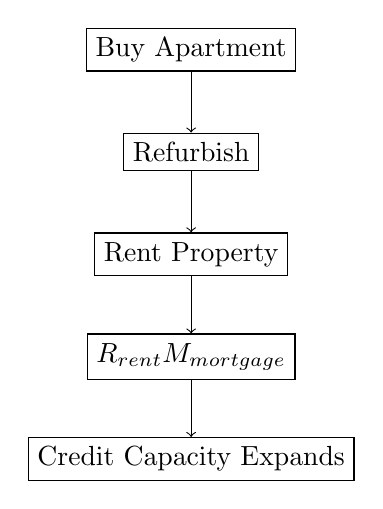
\begin{tikzpicture}
\node[draw, rectangle] (a) at (0,2.4) {Buy Apartment};
\node[draw, rectangle] (b) at (0,1.1) {Refurbish};
\node[draw, rectangle] (c) at (0,-0.2) {Rent Property};
\node[draw, rectangle] (d) at (0,-1.5) {\(R_{\text{rent}} \gtrsim M_{\text{mortgage}}\)};
\node[draw, rectangle] (e) at (0,-2.8) {Credit Capacity Expands};

\draw[->] (a) -- (b);
\draw[->] (b) -- (c);
\draw[->] (c) -- (d);
\draw[->] (d) -- (e);
\end{tikzpicture}
\end{figure}

The lecture then pivots from leverage to education. Asked whether college mattered, the speaker says he went to college but insists that college is not where he got his real information. Instead he names mentorship and family business, and then upgrades the point into a memorable slogan: one needs a PhD in communication. The phrase is obviously rhetorical, but the doctrine underneath it is precise enough:
\begin{equation}
\text{communication skill} + \text{nonreaction} \Rightarrow \text{commercial advancement}.
\end{equation}
Communication here is not presentation polish. It is the ability to handle real people in real time, survive difficult situations, and make adjustments without emotional collapse.

The emotional half of the doctrine is equally strong. He says we must not be reactionary, even when working under people we dislike or when being treated badly. The point is not moral softness; it is career strategy. That yields the companion rule
\begin{equation}
\text{emotional reactivity} \Rightarrow \text{career and business damage}.
\end{equation}
The host's recap after the interview does important work. He takes the longer, messier conversation and compresses it into two final lessons: learn how to communicate, and never show emotion in business.

\subsection{Question \& Answer}

\paragraph{Question.} How does communication become a form of capital that school alone does not supply?

\paragraph{Answer.} Because in the lecture communication is not grammar or polish. It is the practical ability to survive friction, interpret people, adjust in real time, and keep working without emotional collapse. Those capacities alter hierarchy, trust, and opportunity; they behave like productive capital inside a career.

\section{The Trader's Spine: Amazon, Margin Calls, and Access}

The final major interview belongs to an older trader whose family has been in real estate for decades and whose own activity extends into finance and options. His stated horizon markers are:
\begin{equation}
t_{\text{family,start}} = 1945,
\qquad
a_{\text{trader}} \approx 70,
\qquad
t_{\text{college}} \approx 1.5\,\text{years}.
\end{equation}
The lecture first narrows to one successful trade: Amazon. He calls it his cash cow. He then refuses to turn the story into magic. When the host asks what separates the top traders, the answer is determination.

That answer becomes concrete when he introduces mistakes, margin calls, and emotional unreadiness. The transcript around the exact amounts is garbled, and we should not fabricate numbers. But the qualitative structure is clear:
\begin{equation}
\text{leverage} + \text{margin call} + \text{emotional fragility}
\Rightarrow
\text{catastrophic decision risk}.
\end{equation}
He uses the Robinhood anecdote to underline the same point: the danger is not only financial leverage, but psychological unreadiness for the consequences of leverage.

The interview then turns to banks. He says banks want to take money and invest it for clients, but that he prefers doing it himself. The only stable numerical comparison given is the bank-like return band:
\begin{equation}
r_{\text{bank}} \approx 5\%\text{--}6\%.
\end{equation}
He implies that his own trading exceeded that, but refuses to specify how much. We should keep the comparison and not invent a number.

The most mathematically suggestive part comes at the end, when the host asks whose generation works harder. The trader's answer is not merely about work ethic. It becomes a statement about access. Earlier generations were shut out of markets unless they knew the right intermediary. The internet changed that. Small repeated investments are now possible, and over long spans they matter:
\begin{equation}
T \approx 30\text{--}40\,\text{years}.
\end{equation}
The transcript's natural mathematical completion is a compounding model for repeated small contributions:
\begin{equation}
V_T = \sum_{t=1}^{T} c_t(1+r)^{T-t},
\qquad
c_t \sim \$100\ \text{increments}.
\end{equation}
This is not a formula spoken verbatim in the interview, but it is the clean note-writing form of the speaker's point: a hundred dollars here, a hundred dollars there, if kept alive over decades, accumulates into something the young person cannot yet see.

The governing structural implication is
\begin{equation}
\text{internet access} \Rightarrow \text{lower market-entry friction}.
\end{equation}
That is the final pivot of the lecture. The question began as ``whose generation works harder?'' The answer ends up being: the structure of access has changed, and therefore the practical path available to the young has changed with it.

\subsection{Question \& Answer}

\paragraph{Question.} Why does internet access change the wealth-building game for younger entrants?

\paragraph{Answer.} Because it lowers entry friction. The older trader's point is not that technology abolishes risk. It is that participation no longer depends on already belonging to the right institutional network. Small recurring entry becomes feasible, and once that is combined with a \(30\text{--}40\)-year horizon, compounding becomes a real option rather than a remote abstraction.

\section{Summary}

The lecture begins with scale and ends with access. In between, it gives us a sequence of partial rules rather than one grand formula. The construction mogul teaches inspection, diversification, and the negative art of selling. Steve Madden teaches help, capital, product priority, and epistemic humility. The multi-business operator teaches rent-funded leverage, mentorship, communication, and nonreaction. The older trader teaches determination, emotional preparedness under leverage, and the historical significance of internet-era access.

We may compress the chapter into a short chain of implications:
\begin{align}
\text{inspection} &\Rightarrow \text{control},\\
\text{bad deal avoidance} &\Rightarrow \text{better selling},\\
\text{product quality} &\Rightarrow \text{distribution matters},\\
R_{\text{rent}} \gtrsim M_{\text{mortgage}} &\Rightarrow \text{self-carrying leverage},\\
\text{communication} + \text{nonreaction} &\Rightarrow \text{commercial mobility},\\
\text{internet access} + T &\Rightarrow \text{compounding opportunity}.
\end{align}
That is the real mathematical payload of the street format. The interviews look discontinuous on the surface, but taken in order they draw a coherent picture: wealth is built through controlled delegation, selective refusal, product judgment, leverage that carries itself, emotional discipline, and access sustained over time.